\documentclass{standalone}
\usepackage{tikz}
\usepackage{ctex,siunitx}
\setCJKmainfont{Noto Serif CJK SC}
\usepackage{tkz-euclide}
\usepackage{amsmath}
\usetikzlibrary{patterns, calc}
\usetikzlibrary {decorations.pathmorphing, decorations.pathreplacing, decorations.shapes,}
\begin{document}
\small
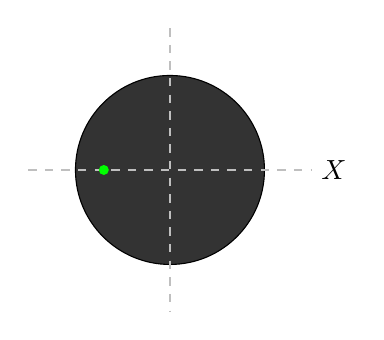
\begin{tikzpicture}[>=latex,scale=1.2]
  % \useasboundingbox(-1,1.2)rectangle(5,2.8);
  \draw [fill=black!80](1.5,0) circle (1);
  \draw [dashed,lightgray] (0,0)--(3,0)node[right,text=black]{$X$};
  \draw [dashed,lightgray](1.5,1.5)--(1.5,-1.5); 
  \fill[green] (.8,0) circle (1.5pt);
  \end{tikzpicture}
\end{document}